\documentclass[10pt,twocolumn]{article}

\usepackage[italian]{babel}
\usepackage[utf8]{inputenc}
\usepackage[T1]{fontenc}
\usepackage{graphicx}
\usepackage{caption}
\usepackage{subcaption}

\usepackage{listings}% http://ctan.org/pkg/listings
\lstset{
  basicstyle=\ttfamily,
  mathescape
}

\usepackage[a4paper,top=0.6cm,bottom=1.8cm,left=2cm,right=2cm]{geometry}

\usepackage{amsmath}
\usepackage{graphicx}

\usepackage[backend=biber]{biblatex}
\addbibresource{ref.bib}

\title{\textbf{Progettazione e realizzazione di un algoritmo di Voice Activity Detection}}

\author{Giacomo Camposampiero, matricola 1187180}

\begin{document}
\maketitle

\section{Introduzione}
{Gli algoritmi di \textit{Voice Activity Detection} (VAD) sono algoritmi sviluppati allo scopo di rilevare la
presenza o l'assenza di voce umana all'interno di segnali audio. Questi algoritmi trovano applicazione in una vasta gamma di sistemi per l'elaborazione del suono e per la comunicazione audio real-time. In questi ultimi in particolare i sistemi VAD si rivelano molto efficaci nella riduzione dell'informazione media trasmessa tra utenti, essendo i silenzi una componente non marginale nella maggior parte delle conversazioni umane.

\vspace{0.1cm}
La letteratura scientifica è al giorno d'oggi ricca di metodi, proposti dalla comunità scientifica nel corso
degli ultimi anni, per l'implementazione di un Voice Activity Detector. 
In questo lavoro ne sono stati selezionati alcuni allo scopo di implementare un classificatore per
l'identificazione del parlato in un segnale audio digitale mono, codificato mediante una modulazione ad impulsi
codificati (PCM, dall'inglese \textit{Pulse-Code Modulation}) e pacchettizzati dal trasmettitore in pacchetti di
160 campioni audio. La classificazione è eseguita con lo scopo di decidere quali pacchetti trasmettere
(perché contenenti voce, a cui si farà di seguito riferimento con la sigla \textsl{ACTIVE}) e quali invece
scartare perché privi di contenuto vocale (\textsl{INACTIVE}). 
Gli obiettivi del classificatore comprendono la massimizzazione della compressione del
segnale, la minimizzazione del clipping nel segnale vocale e il mantenimento del ritardo sotto una soglia
massima di 50ms. 

\section{Descrizione del metodo}
Come già accennato in precedenza, l'approccio alla risoluzione della consegna che si è voluto adottare è stata
la creazione di un \textit{ensemble} di classificatori. Essendo i metodi utilizzati poco elaborati, raggiungere
elevate prestazioni mediante l'uso di uno solo di essi è stato infatti verificato essere molto meno efficace 
rispetto al loro utilizzo parallelo. I metodi che si è deciso di includere sfruttano due tipi di analisi del segnale:
\begin{itemize}
\item \textbf{analisi nel dominio del tempo}, che deriva la presenza di voce dalle ampiezze del suono
\item \textbf{analisi nel dominio della frequenza}, che deriva la presenza di voce a partire dallo studio in frequenza del segnale
\end{itemize}
In Figura (\ref{fig:diag}) è riportato il diagramma di flusso del metodo proposto; l'implementazione di quest'ultimo è stata svolta in Matlab. Ognuno dei singoli approcci inclusi nell'ensemble viene trattato più nel dettaglio nelle sezioni successive. 

\begin{figure}[h!]
	\centering
	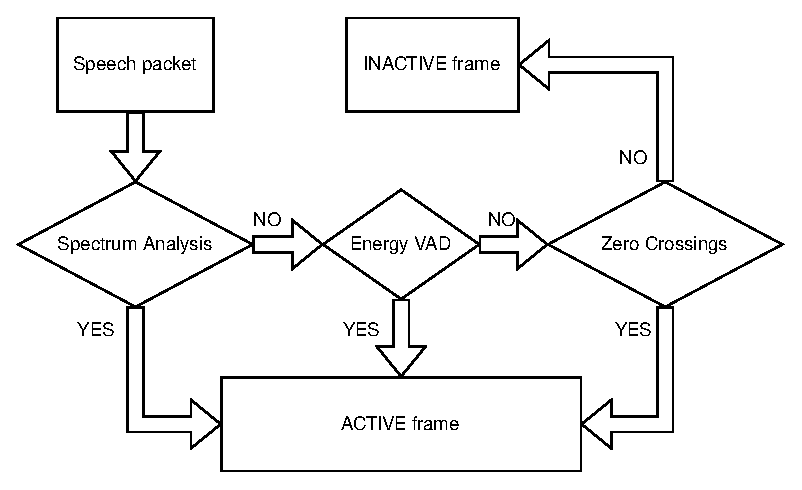
\includegraphics[scale=0.65]{images/diagram.eps}
  	\caption{Flow chart dell'implementazione di VAD proposta.}
  	\label{fig:diag}
\end{figure}

\subsection{Linear energy-based detector}
\label{sect:led}
{Il \textit{Linear Energy-based detector} è stato il primo tipo di classificatore implementato in questo progetto. Si tratta di un classificare basato sull'analisi nel dominio del tempo, che classifica un frame in base alla sua energia. L'energia di un frame può essere calcolata come}
\begin{align*}
E_{frame} = \frac{1}{n} \, \sum_{i=1}^{n} x^2(i)
\end{align*}
dove $n$ è il numero di campioni del frame e $x(i)$ il campione $i$-esimo del frame. La decisione sul tipo di frame viene effettuata secondo la regola
\begin{quote}
\begin{lstlisting}
IF ($E_{frame}$ > k$\cdot E_s$) ACTIVE
ELSE INACTIVE
\end{lstlisting}
\end{quote}
\vspace{-0.2cm}
dove $E_s$ equivale all'energia media dei frame INACTIVE e $k$ è un iperparametro del metodo di classificazione.

\vspace{0.1cm}
Una stima iniziale dell'energia media dei frame INACTIVE è fatta lavorando nella verosimile ipotesi che i primi
10 frame (corrispondenti a 200ms) della trasmissione non abbiano contenuto vocale. Il valore di questa soglia
viene poi aggiornato ad ogni nuovo frame classificato come INACTIVE secondo la relazione
\begin{align}
E_s = E_s \cdot (1-p) + E_{frame} \cdot p
\label{eq:upd}
\end{align}
dove $E_{frame}$ è l'energia del frame appena classificato e $p$ un dato valore di probabilità che regola la
velocità di aggiornamento del valore di soglia.

Il principale vantaggio di questo algoritmo risiede nella sua facilità di implementazione. Questa tecnica
risulta tuttavia essere inefficiente nel caso di rumore di fondo altamente variabile o di SNR 
(\textit{Signal to Noise Ratio}) basso. 
\pagebreak

\newgeometry{top=1.6cm,bottom=1.8cm,left=2cm,right=2cm}
\subsection{Zero crossings detector}
Un secondo metodo di classificazione implementato al fine di migliorare le prestazioni del
precedente, soprattutto nel caso di segnali a bassa energia, è basato sul numero di 
\textit{zero crossing}. Tale valore è pari al numero di volte in cui il segnale interseca
l'asse delle ascisse in un dato intervallo temporale. Il numero di crossing di un frame ACTIVE è contenuto
in un range fisso che, nel caso di un frammento ACTIVE di 10ms, è all'incirca pari a $[5,15]$. 
Nel caso di frame INACTIVE, al contrario, il numero di zero crossings è totalmente casuale. 
Per sua stessa definizione, anche questo metodo esegue un'analisi del segnale nel dominio del tempo.

\vspace{0.1cm}
Questo ci permette quindi di definire una regola di decisione completamente indipendente dall'energia del frame
in analisi e che, di conseguenza, è in grado di identificare frammenti di parlato a bassa energia con maggior
facilità. La regola sulla base di cui è definito il metodo equivale a
\begin{quote}
\begin{lstlisting}
IF ($N_{zc} \in R$ ) ACTIVE
ELSE INACTIVE
\end{lstlisting}
\end{quote}
dove $N_{zc}$ equivale al numero di zero crossing in un dato pacchetto e $R$ è l'intervallo in cui dovrebbe ricadere lo stesso per essere classificato come voce.

\vspace{0.1cm}
Anche in questo caso uno dei principali vantaggi dell'approccio consiste nella facilità di implementazione. Di
contro, l'approccio risulta essere in alcuni casi impreciso a causa della forte casualità nel numero di crossing
di segnali diversi dalla voce umana.

\subsection{Linear Sub-Band Power Detector}
L'ultimo approccio implementato è basato invece su di un'analisi in frequenza della potenza del segnale in ingresso. In particolare, i frame che comprendono un contenuto vocale sono caratterizzati da potenze nella
banda $1Hz$-$1kHz$ più grandi rispetto a frame che contengono invece silenzi o rumori di fondo. Al fine di
ottenere lo spettrogramma e le relative potenze del segnale è stato utilizzato il metodo \texttt{pspectrum()}
fornito da Matlab.

\vspace{0.1cm}
La decisione sul tipo di frame viene quindi effettuata secondo la regola
\begin{quote}
\begin{lstlisting}
IF ($P_{frame}$ > k$\cdot P_s$) ACTIVE
ELSE INACTIVE
\end{lstlisting}
\end{quote}
\vspace{-0.2cm}
dove $P_s$ equivale alla potenza media dei frame INACTIVE e $k$ è un iperparametro del metodo di classificazione.
Come per il classificatore tratta nella Sezione \ref{sect:led}, una stima iniziale della potenza media dei frame INACTIVE è fatta lavorando nella verosimile ipotesi che i primi
10 frame della trasmissione non abbiano contenuto vocale. 
Il valore di questa soglia viene anche in questo caso dinamicamente aggiornato secondo una relazione simile a (\ref{eq:upd}).

Questo tipo di approccio è quello che, preso singolarmente, riesce ad ottenere i risultati migliori, non dipendendo di fatto dall'energia della voce ma solamente dalle sue componenti in frequenza. 

\subsection{Finestra scorrevole}
Al fine di migliorare le prestazioni dell'algoritmo è stato implementato un sistema a finestra scorrevole,
in cui la classificazione di ogni pacchetto è eseguita sulla base del pacchetto stesso, del precedente e di quello successivo. Questo ha permesso di ridurre sensibilmente il clipping sulla voce e rendere più
fluido il risultato finale, pur mantenendo un ritardo totale inferiore alla soglia limite. 

\section{Risultati}
{Sono riportati in Figura (\ref{fig:results}) i risultati della simulazione per i 5 file di test forniti dalla consegna. Nei grafici di seguito la componente di colore nero corrisponde alle porzioni di segnale appartenenti a pacchetti classificati come ACTIVE, che verrebbero quindi trasmessi dalla sorgente. La componente di colore rosso corrisponde invece alle porzioni classificate come INACTIVE, che verrebbero scartate e non trasmesse dalla sorgente.}

\begin{figure}[ht]
  \centering
  \begin{subfigure}{0.45\linewidth}
    \centering
    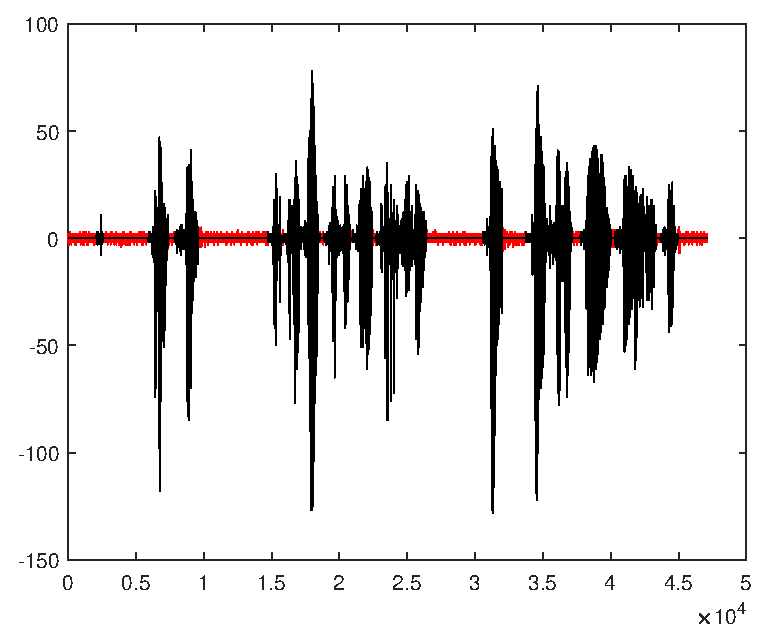
\includegraphics[scale=0.3]{images/res1.eps}
    \caption{inputaudio1.data}
  \end{subfigure}
\begin{subfigure}{0.45\linewidth}
    \centering
    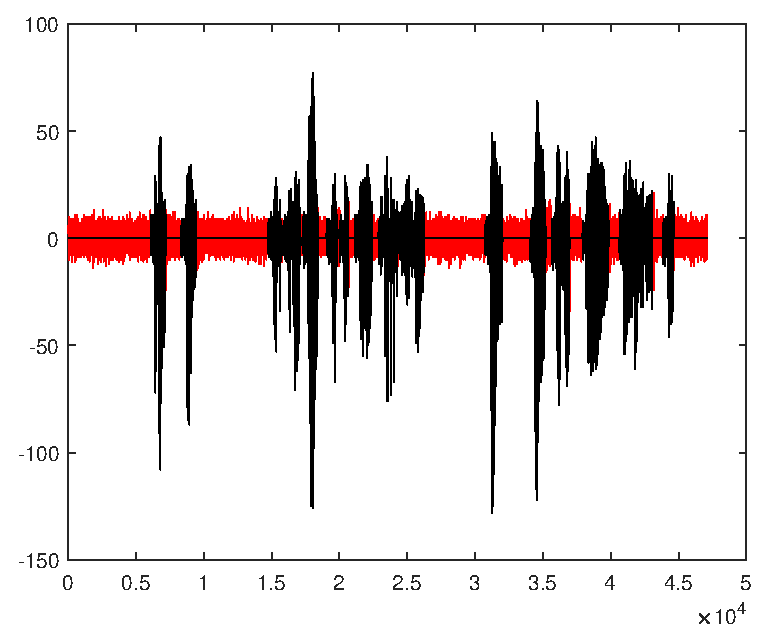
\includegraphics[scale=0.3]{images/res2.eps}
    \caption{inputaudio2.data}
  \end{subfigure}
  \par\medskip
  \begin{subfigure}{0.45\linewidth}
    \centering
    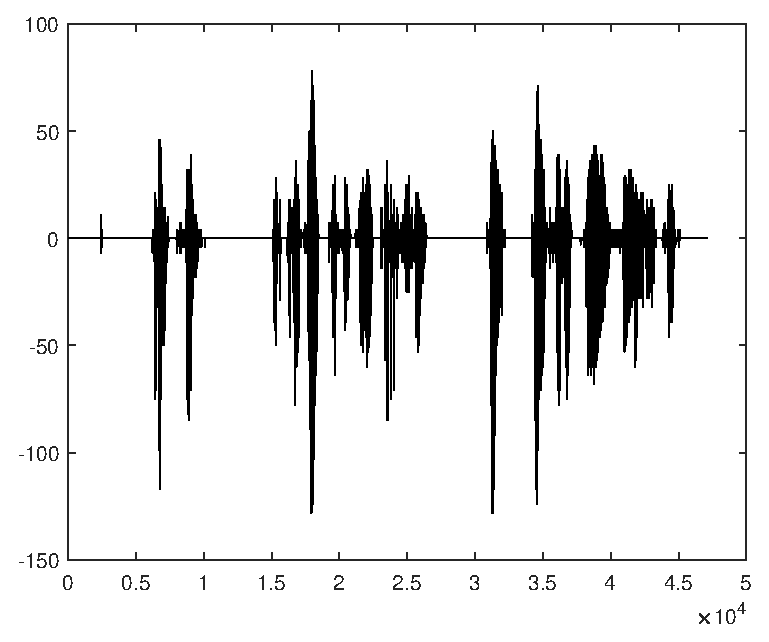
\includegraphics[scale=0.3]{images/res3.eps}
    \caption{inputaudio3.data}
  \end{subfigure}
  \begin{subfigure}{0.45\linewidth}
    \centering
    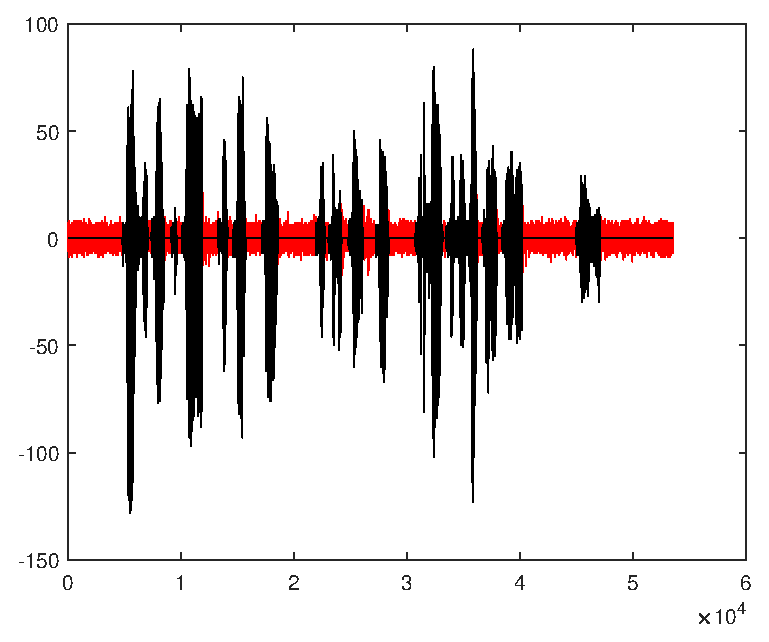
\includegraphics[scale=0.3]{images/res4.eps}
    \caption{inputaudio4.data}
  \end{subfigure}
  \par\medskip
  \begin{subfigure}{0.45\linewidth}
    \centering
    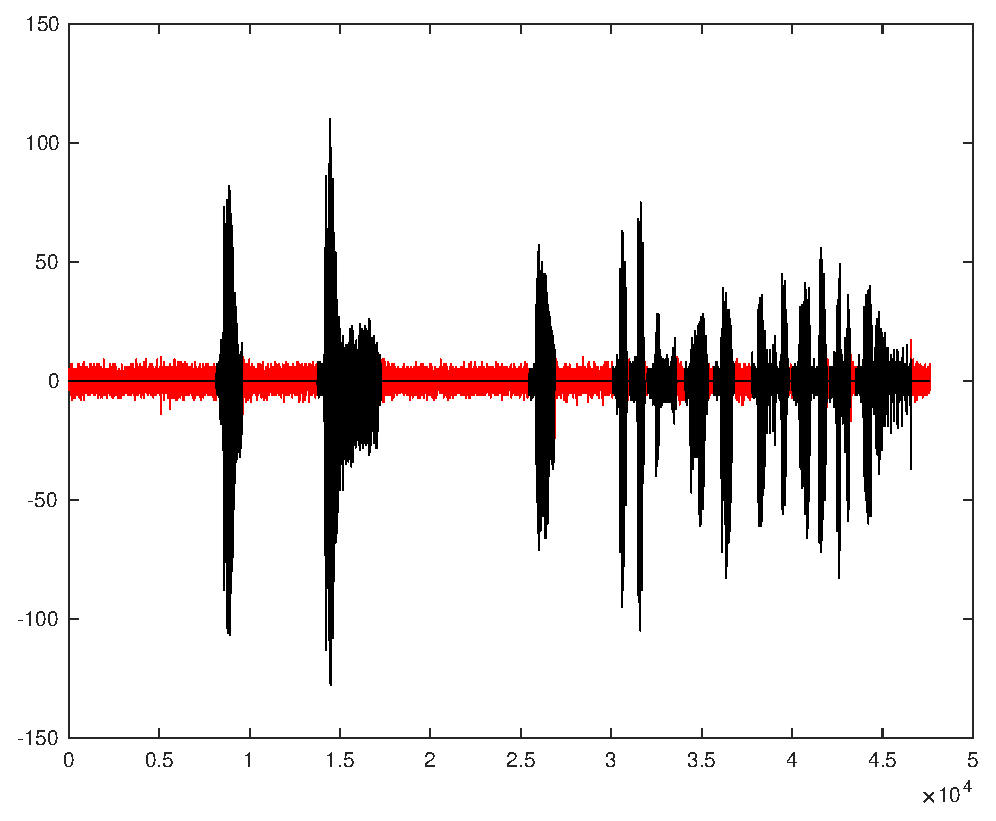
\includegraphics[scale=0.25]{images/res5.eps}
    \caption{inputaudio5.data}
  \end{subfigure}
  \caption{Risultati dell'applicazione dell'algoritmo implementato alle tracce di test.}  
  \label{fig:results}
\end{figure}  

\vspace{-0.5cm}
\section{Conclusioni}
Il metodo proposto per l'implementazione di un VAD restituisce risultati che, almeno per le tracce audio di test, si considerano essere soddisfacenti. Tuttavia, il metodo proposto rappresenta 
un'implementazione estremamente basilare e potrebbe, in presenza di rumori di fondo fortemente variabili
o eterogenei o nel caso di SNR estremamente ridotto, risultare meno efficace nella classificazione dei pacchetti. 

\end{document}